\section{Conclusion}

This project have been a textbook example of an iterative process of improving results one parameter at a time, with methods including both numerical predictions and an experimental trial-and-error approach. We have been able to achieve an almost complete overlap between the Fano theory for a plane-wave and the recorded data, and while broadening is still present in the resonance transmission spectra, I confidently conclude that the double Fano model have been succesfully realized. 

Using suspended $SiN$ membranes patterned with sub-wavelength gratings, utilized as $TM_0$ waveguides, we have succesfully displayed an enhanced spectral sensitivity compared with a single Fano cavity of similar losses for short cavities, i.e. inside the Fano regime. It has been shown numerically that the double Fano cavity has the potential to produce linewidths similarly narrowed even for longer cavities, and the outlook of achieving this experimentaly is believed to belong in the near future. 

The general behavior of the double Fano cavity has been thoroughly examined and documented through numerical simulations, once again assuming an incident plane-wave. The analytical model describing the linewidth of single- and double Fano cavities have likewise been studied and verified through both experimental and numerical results. 

The realization of the double Fano cavity provides promise for a number of potential applications. These include, but are not limited to Fano cavity optomechanics, optical sensing and Fano lasers, and will be briefly outlines individually in the outlook section  below. 

\subsection{Outlook}

\subsubsection{Matching analytical and experimental linewidths}

I believe that the task of matching the analytical linewidth of the double Fano resonance transmission spectra with experimental data is one that consists of improving the method used and attempting to isolate the setup from vibrational noise stemming from outside sources. For this reason it is believed that this outlook is one that will be fulfilled in the near future. 

\subsubsection{Optomechanics with the double Fano cavity}

This project have been dealing exclusively with the optical properties of the Fano mirrors. They are however often chosen for experiments in the field of cavity electrodynamics for their remarkable mechanical properties displaying high mechanical quality factors. Inside the Fano regime where the double Fano cavity linewidth is much narrower than for a similar broadband cavity of the same length, the radiation pressure is also high enough to excite mechanical modes in the high-Q $SiN$ membranes. If placed inside a vacuum, the double Fano cavity is therefore an obvious candidate for studying optomechanial effects, e.g. the optical spring effect\cite{Manjeshwar}.

\subsubsection{Sensing applications of the double Fano cavity}

Various sensing applications using the bare $SiN$ membranes are already being studied extensively. The isothermic compression of a gas in the free molecule regime inside a so-called membrane "sandwich" modifies the mechanical properties of the membranes due to the \emph{squeeze film effect}. Figure \ref{fig:squeeze_film_pressure_sensor_sketch} shows an example as a simple sketch of a double Fano cavity in a membrane "sandwich" configuration which can be utilized to measure absolute vapor pressure\cite{Salimi}. The change in mechanical properties of the Fano mirrors can then be recorded optically\cite{Al-Sumaidae,Hornig}. 

\begin{figure}[h!]
    \centering
    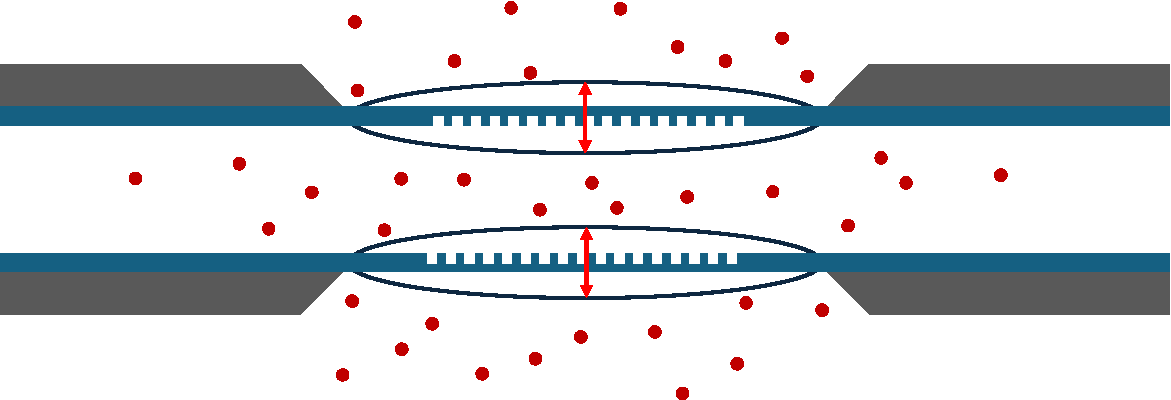
\includegraphics[width=0.7\textwidth]{figures/squeeze_film_pressure_sensor_sketch.pdf}
    \caption{}
    \label{fig:squeeze_film_pressure_sensor_sketch}
\end{figure}

\subsubsection{Fano laser based on bound states in the continuum}

Firstly, a bound state in the continuum (BIC) is a state that remains localized while existing alongside a continuous spectrum of states that can provide and take away energy. They defy the general idea that states are either discrete or exist in a continuum. They are a relatively new discovery in the field of quantum mechanics, but have since been discovered to exist as a general wave phenomenon and can thus be utilized in numerous applications\cite{Hsu}. 

It has been proposed to utilize these BICs based on interference inside a cavity closely related to the double Fano cavity. This principle would allow for the construction of an ultra-coherent nanoscale laser, combating the limitation of quantum fluctuations, with potential applications in on-chip communication, photonic integrated circuits, bio/chemical sensing and quantum computing\cite{Yu}. 

